\documentclass[14pt]{article}
\usepackage[utf8]{inputenc} 
\usepackage[T1]{fontenc} 
\usepackage{xcolor}
\usepackage[english,ukrainian]{babel}
\usepackage{tempora}
\usepackage{lipsum}
\usepackage{setspace}
\usepackage{geometry}
\usepackage{graphicx}
\graphicspath{ {./images/} }
\geometry{a4paper, total={170mm,257mm}, left=20mm, top=20mm,}
\pagenumbering{arabic}


\begin{document}
\begin{spacing}{1.175}	
	\begin{titlepage} 
		\newcommand{\HRule}{\rule{\linewidth}{0.3mm}}
		\center 
		
		\textsc{\large Національний технічний університет України
			\\"Київський політехнічний інститут імені Ігоря Сікорського"}\\[1.5cm]
		
		\vspace{5cm}
		\textsc{\large Теорія складності}\\[0.5cm]
		
		\textsc{\large Дослідження \(coNP\)-повної задачі}\\[0.5cm] 
		
		\HRule\\[0.4cm]
		
		{\huge \textcolor{blue}{Проблема негамільтонового циклу}}\\[0.4cm]
		
		\HRule\\[1.5cm]
		\textsc{\large ФІ-13 Дідух Максим}\\[0.5cm]
		
		\vspace{7.5cm}
		
		\textsc{\large Фізико-технічний інститут}\\[0.5cm]
		\textsc{\large Кафедра математичних методів захисту інформації}\\[0.5cm]
		{\large {2022}} 
	\end{titlepage}
    
    
    
    \newpage
    \title{\Large Дослідження \(coNP\)-повної задачі}
    \date{\large 7 грудня 2022}
    \maketitle
    \tableofcontents                                                                            %CHANGE THICKNESS HERE AND IN NUMBERING))))0)
    \newpage
    \section{\normalfontВступ}
        \quadГраф \(G\) називається \textit{гамільтоновим}, якщо існує цикл, що містить кожну вершину рівно один раз. Такий цикл носить назву гамільтонового. Також слід зазначити, що існує поняття гамільтоновго шляху (це знадобиться при доведенні складності): граф \(G\) має \textit{гамільтонів шлях} з вершини \(s\) у вершину \(t\), якщо є марштрут між цими вершинами, який містить усі вершини рівно один раз.
        
        \\
        \quad Взагалі, це поняття пішло від Вільям Гамільтон (англ. \textit{William Hamiltonian}), який вигадав не дуже вдалу гру під назвою "ікосіанська гра" (англ. \textit{"icosian game"}), завданням якої був пошук гамільтонового циклу на додекаедричному графі (і можливо на його підграфах). \\
        \begin{center}
        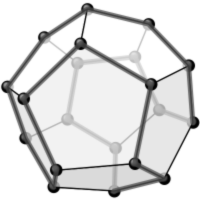
\includegraphics{images/dod(200x200)-modified.png} \\
        \text{мал. 1 \textit{гамільтоновий цикл на додекаедрі} \textcolor{blue}{\large change resolution}}
        \end{center}
        
        \parХоча означення гамільтонового графу дуже схоже з означенням ойлерового графу, виявляється, що ці дві концепції поводяться досить по-різному. Якщо теорема Ойлера дає нам чіткий критерій ойлеровості, то для гамільтонових графів немає аналогічного твердження. Як з'ясувалось, перевірка графу на наявність гамільтонового циклу є \(NP\)-повною задачею.

        \newcommand{\nonhamcycle}{\textit{NON-HAM-CYCLE }}
        \newcommand{\hamcycle}{\textit{HAM-CYCLE }}
        \newcommand{\dhampath}{\textit{D-HAM-PATH }}
        \newcommand{\tsat}{\textit{3SAT }}

        
        \subsection{\normalfontПостановка задачі}
        \quad Дано: неорієнтований граф \(G = (V,E)\), де \(V = \{v_1, v_2, \dots v_n\}\) - множина вершин, \(E\ = \{e_1, e_2, \dots v_k\}\) - множина ребер. Перевірити, що даний граф не має циклу гамільтона. Цю задачу будемо позначати \nonhamcycle .    
        \subsection{\normalfont Історичний екскурс}
        \textcolor{blue}{НЕ ПОДОБАЄТЬСЯ}
        
        Проблема негамільтонового циклу (\nonhamcycle) — це математична задача, яка існує з кінця 1960-х років, що передбачає перевірку графа на не наявність циклу гамільтона, але наявність усіх інших циклів. Проблема була вперше поставлена в 1969 році Вільямом Тутте і Річардом Тістлетвейтом і стала областю активних досліджень як у математиці, так і в інформатиці.

        \nonhamcycle можна розглядати як узагальнення класичної проблеми гамільтонового циклу. У цій узагальненій версії ми хочемо знайти цикли на довільному графі, які не є гамільтоновими, але допускаються всі інші цикли довжиною не менше трьох. \nonhamcycle має низку застосувань у галузі теорії графів і суміжних областях, таких як оптимізація мережі, планування та проектування схем. Крім того, проблема має значення для вивчення орієнтованих графів, оскільки вона служить схемою для створення негамільтонових циклів у орієнтованих графах.

        Дивно, але незважаючи на те, що \nonhamcycle було запропоновано понад 50 років тому, незначний прогрес був досягнутий у пошуку алгоритму поліноміального часу. Відомо, що проблема NP-Hard; проте було розроблено низку евристичних та апроксимаційних алгоритмів, у тому числі на основі локального пошуку, ланцюга Маркова Монте-Карло та генетичних алгоритмів.

        Проблема негамільтонового циклу все ще залишається головним відкритим питанням у теоретичній інформатиці та математиці. Хоча за останні роки було досягнуто значного прогресу, все ще потрібно багато працювати, щоб визначити, чи можна розв’язати проблему за поліноміальний час. Тим часом дослідження цієї захоплюючої проблеми продовжують надихати математиків, комп’ютерників та інженерів із різних галузей.
    
    \section{\normalfontПрактичне застосування}
    Негамільтонові цикли мають широкий спектр застосування, оцінити вплив цього поняття та теорії, що побудувалась навколо нього неможливо, тому я спробую навести лише деякі (очевидні та не дуже) приклади застосування:
    \begin{itemize}
       
        \item Мережі
        \begin{itemize}
            
            \item Проектування мереж: негамільтонові цикли можна використовувати для проектування надійних мереж, у яких існує кілька надлишкових шляхів між двома точками в мережі.
        
            \item Проектування мережі: негамільтонові цикли часто використовуються при проектуванні мереж, де метою є створення шляху, який відвідує всі вузли мережі, не проходячи через жодний вузол більше одного разу.
        
            \item Маршрутизація: негамільтонові цикли можна використовувати для маршрутизації інформації через мережу комп’ютерів. Це особливо актуально для комп’ютерних мереж, які містять вузли з різною потужністю або функціями. У цьому випадку можна використовувати негамільтонів цикл, щоб знайти шлях через мережу, який використовує переваги окремих вузлів, мінімізуючи затримку та перевантаження.
        
            \item Маршрутизація: негамільтонові цикли зазвичай використовуються в алгоритмах мережевої маршрутизації, таких як алгоритм Беллмана-Форда, який знаходить найкоротший шлях між двома вузлами в мережі, спочатку будуючи негамільтонів цикл.
            
            \item Проектування мереж: негамільтонові цикли можна використовувати для створення ефективних мереж, таких як комунікаційні мережі, транспортні мережі та ланцюги поставок. Використовуючи підхід негамільтонового циклу, ці мережі можуть бути більш ефективними, ніж традиційні гамільтонові цикли.
            
        \end{itemize}


        \item Аналіз даних
        \begin{itemize}
            
            \item Аналіз даних: негамільтонові цикли можна використовувати для виявлення закономірностей у наборах даних, допомагаючи визначити зв’язки між різними частинами даних.
            
            \item Машинне навчання: негамільтонові цикли також використовуються в алгоритмах машинного навчання, таких як нейронні мережі та опорні векторні машини, для визначення закономірностей і прогнозування.
                
            \item Візуалізація даних: негамільтонові цикли корисні для візуалізації даних у формі графіків, наприклад, коли використовується силово-спрямований алгоритм компонування графа \textit{(force-directed graph layout algorithm)}. Такі алгоритми, використовують концепцію сил «відштовхування» та «притягання» для розташування вузлів у межах графа. Гамільтонів цикл не обов’язково є ідеальним для такого виду візуалізації, оскільки його ребра можуть стати занадто стиснутими, якщо є лише кілька вузлів або якщо вузли розташовані дуже близько один до одного. Негамільтонові цикли забезпечують більшу гнучкість і краще підходять для відображення складних даних у візуально цікавий та інформативний спосіб.

            \item Розпізнавання шаблонів: негамільтонові цикли можна використовувати для пошуку шаблонів або трендів у великих наборах даних.
        
        \end{itemize}


        \item Криптографія
        \begin{itemize}
             
             \item Негамільтонові цикли також використовуються в певних криптографічних системах, таких як обмін ключами Діффі-Хеллмана та криптографія еліптичної кривої, для безпечної передачі даних через Інтернет.
        
        \end{itemize}


        \item Планування та логістика
        \begin{itemize}
            
            \item Планування: негамільтонові цикли можна використовувати для планування завдань у розподілених системах, оскільки вони забезпечують ефективний спосіб мінімізації загального часу, необхідного для виконання всіх завдань.

            \item Планування: негамільтонові цикли можна використовувати для планування завдань на паралельному процесорі, наприклад планування завдань на роботі-мануалі на виробничому підприємстві.
            
            \item Планування: негамільтонові цикли можна використовувати для створення оптимальних розкладів для складних завдань, таких як планування маршрутів польоту або оптимізація операцій ланцюга поставок.
            
            \item Оптимізація логістики: негамільтонові цикли можна використовувати для вирішення проблеми комівояжера в оптимізації логістики, де метою є знайти найкоротший маршрут для транспортного засобу доставки серед кількох зупинок.

            \item Планування шляху: негамільтонові цикли також можна використовувати для планування шляху, особливо коли на шляху є перешкоди. Цикл можна використовувати для уникнення цих об’єктів під час пошуку найкоротшого маршруту між двома точками.

            \item Маршрутизація транспортного засобу: негамільтонові цикли можна використовувати в задачах маршрутизації транспортного засобу, де метою є знайти найефективніший маршрут для руху транспортного засобу між набором місць.
        
        \end{itemize}

            
        \item Обробка зображень
        \begin{itemize}
    
            \item Обробка зображень: алгоритми на основі графів з негамільтоновими циклами використовуються при сегментуванні зображень на області чи об’єкти.
            
            \item Обробка зображень: негамільтонові цикли також використовуються в задачах обробки зображень, таких як виявлення країв на зображеннях і визначення форм на цифрових фотографіях.

            \item Мистецтво та дизайн: негамільтонові цикли можна використовувати для створення естетично привабливих візерунків у мистецтві та дизайні.
        
        \end{itemize}
        
        \item Робототехніка
        
        \begin{itemize}
            \item Роботна навігація: негамільтонові цикли створюють основу для досліджень певного середовища роботами, одночасно уникаючи перешкод.

            \item Робототехніка: роботи можуть використовувати негамільтонові шляхи для пересування з місця на місце, уникаючи перешкод і досліджуючи навколишнє середовище.
        
        \end{itemize}


        \item Розфарбування графів
        \begin{itemize}
            
            \item негамільтонові цикли можна використовувати в алгоритмах розфарбовування графів, де метою є розфарбувати всі вершини графа без будь-яких двох суміжних вершин, які мають однаковий колір.

             \item негамільтонові цикли можна використовувати в задачах розфарбовування, щоб розділити граф на два або більше менших підграфів з оптимізованим балансом кольорів.
        
        \end{itemize}


        \item Інше
        \begin{itemize}
            
            \item Промислові процеси: негамільтонові цикли використовуються в промислових процесах, таких як хімічне машинобудування та автоматизація. Наприклад, їх можна використовувати для оптимізації маршрутів постачання матеріалів і виробництва на заводах.

            \item Секвенування ДНК: негамільтонові цикли використовуються в алгоритмах секвенування ДНК. Алгоритми використовують підхід негамільтонового циклу для аналізу відносних положень нуклеотидів у молекулі ДНК.

            \item Проблеми оптимізації: негамільтонові цикли також можна використовувати для вирішення проблем оптимізації, таких як проблема комівояжера. На відміну від рішення, яке ґрунтується на гамільтоновому циклі, який гарантовано знаходить оптимальне рішення, але є дорогим з точки зору обчислень, негамільтонів цикл часто можна використовувати для знаходження майже оптимального рішення за менший час.
        
        \end{itemize}
    \end{itemize}
    

    
    
    \section{\normalfontДоведення складності}
    \quad Доведемо, що \nonhamcycle є \(coNP\)-повною. Для цього нам знадобиться довести додаткове твердження. \\\\
    \textbf{Твердження 1:} задача перевірки графа на наявність гамільтонового циклу належить класу \(NP\)-повних задач (\textit{далі:} \hamcycle)\\
    \rule{0.7em}{0.7em}\\
    Спочатку покажемо, що задача перевірки орієнтованого графу на наявність гамільтоновго шляху з вершини \(s\) у вершину \(t\) (далі \dhampath)  є \(NP\)-повною.
    \\ 
    
    \quad 1. \dhampath \(\epsilon\) \(NP\)-повна?\\
    Нехай \(G\) — орієнтований граф. Ми можемо перевірити чи потенційний шлях \(s \to \dots \to t\) є гамільтоновим за поліноміальний час. Тепер спробуємо побудувати поліноміальне зведення \tsat \(\le_p\) \dhampath, щоб закінчити доведення повноти.
    \\
    \textcolor{blue}{а точно 'множник'?}\\
    Нехай \(\phi = \bigwedge_{i=1}^{m} \phi_{i}\) має \(n\) змінних і \(m\) множників. Щоб спростити доведення, припустимо, що жоден множник в \(\phi\) не містить змінної \(x_i\) і її заперечення \(\bar{x_i}\).  
    
    \begin{enumerate}
        \item  Спочатку, для кожної змінної \(x_i\), ми генеруємо \(2m+1\) вершину з назвою \(v_{i,j}\) і додаємо орієнтовані ребра (\(v_{i,j}\), \(v_{i,j+1}\)) і (\(v_{i,j+1}\), \(v_{i,j}\)), для \(0 \le j \le 2m\).
        
        \item  Далі ми з’єднуємо вершини, пов’язані з різними змінними, додаючи чотири спрямовані ребра (\(v_{i,0}\), \(v_{i+1,0}\)), (\(v_{i,0}\), \(v_{i+1,2m+1}\)), (\(v_{i,2m+1}\), \(v_{i+1,0}\)) та (\(v_{i,2m+1}\), \(v_{i+1,2m+1}\)).
        
        \item  Далі створюємо вершини під назвою \(c_{j}\). Якщо \(x_i\) з'являється у множнику \(\phi_{j}\) без доповнення, додаємо орієнтовані ребра
        (\(v_{i,2j-1}\), \(c_{j}\)) та (\(c_{j}\), \(v_{i,2j}\)). Інакше, якщо \(x_i\) міститься з доповненням, то додаємо орієнтовані ребра (\(v_{i,2j}\), \(c_{j}\)) та (\(c_{j}\), \(v_{i,2j-1}\)).
        
        \item В кінці, ми додаємо дві додаткові вершини \(s\) і \(t\). Після цього додаємо нові ребра (\(s\), \(v_{1,1}\)), (\(s\), \(v_{1,2m+1}\)), \\(\(v_{n,1}\), \(t\)) та (\(v_{n,2m+1}\), \(t\)). Граф згенерований \(G_{\phi}\) (\textit{див. рис.2}). \textcolor{blue}{add picture number2}        
    \end{enumerate}
    \\

    \quad Тепер, треба показати, що \(\phi\) задовільна тоді та лише тоді, коли у графі \(G_{\phi}\) є гамільтонів шлях з \(s\) у \(t\). Припустимо, що \(\phi\) - задовільна. Тоді ми можемо відвідати кожну вершину починаючи з \(s\) йдучи з \(v_{i,0}\) до \(v_{i,2m+1}\) з ліва на право, якщо \(x_i\) - позитивна, і з \(v_{i,2m+1}\) до \(v_{i,0}\) з права на ліво, якщо \(x_i\) - негативна, і закінчити в \(t\) після відвідування \(v_{n,0}\) або \(v_{n,2m+1}\). Крім того, кожна \textcolor{blue}{'clause'} вершина може бути відвідана, згідно з припущенням, що кожна \textcolor{blue}{'clause'} \(\phi_{i}\) має декілька літерлів \(l_i = x_k\) або \(l_i = \bar{x_i}\), які є позитивними. Кожна вершина \(c_j\) може бути відвідана використовуючи ребра (\(x_{k,2j-1}\), \(c_{j}\)) або (\(c_{j}\), \(x_{k,2j}\)) у першому випадку, і (\(x_{k,2j}\), \(c_{j}\)) і (\(c_{j}\), \(x_{k,2j-1}\)) у другому випадку, оскільки шлях йде вправо на графі для позитивних змінних, і шлях йде вліво для негативних змінних. Тому \(G_{\phi}\) має гамільтонів шлях, якщо \(\phi\) задовільна.
    
    \\
    \quad І навпаки, припустимо, що \(G_{\phi}\) має гамільтонів шлях (\(s, t\)), позначимо його \(P\). Зазначимо, що \(G_{\phi}\) без \textcolor{blue}{clause vertices}  є гамільтоновим, тому нам потрібно показати, що шлях не "заламається" після відвідування \textcolor{blue}{clause vertex}. Якщо більш формальніше: потрібно показати, що якщо \(P\) відвідує \(v_{i, 2j-1}\), \(c_j\), \(v\) у відповідному порядку, тоді \(v = v_{i,2i}\). Нехай \(v \neq v_{i,2i}\). Тоді зазначимо, що єдиними вершинами, які входять в \(v_{i,2j}\) є \(v_{i,2j-1}\), \(c_j\), \(v_{i,2j+1}\), а виходять з нього лише \(v_{i,2j-1}\) та \(v_{i,2j+1}\). Тому \(v_{i,2j}\) має бути відвідана з \(v_{i,2j+1}\), але тепер шлях замається і не може продовжуватись, оскільки \(v_{i,2j-1}\) вже відвідано. Аналогічний аргумент показує, що \(P\) відвідує \(v_{i, 2j}\), \(c_j\), \(v\) у відповідному порядку, тому \(v = v_{i,2j-1}\). Отже, гамільтонів шлях в \(G_{\phi}\) відвідує вершини в порядку від \(x_1\) до \(x_n\), чергуючи \textcolor{blue}{clause vertices} вершини між змінними , пов'язаними з тією самою змінною. Тому, значення змінних \(x_i\) добре визначається, якщо помітити, у якому напрямку шлях йде через вершини \(x_i\) у графі \(G_{\phi}\). За побудовою це присвоєння буде задовільняти \(\phi\), оскільки воно робити літерал у кожній \textcolor{blue}{clause} позитивним. \textcolor{blue}{fix brackets bug}
    
    \\
    \quad Зведення відбувається за \(O(mn)\) час, який є поліномом довжини вхідних даних.
    \\


    \\
    \quad 2. \hamcycle \(\epsilon\) \(NP\)?\\
        Якщо довільна задача, належить класу \(NP\), тоді, маючи «сертифікат», який є розв'язком зієї задачі та екземпляр проблеми (граф \(G\) і додатне ціле \(k\), у цьому випадку), ми зможемо верифікувати ( перевірити, чи надане рішення правильне чи ні) сертифікат за поліноміальний час. Сертифікат — це послідовність вершин, що утворюють гамільтонів цикл у графі. Ми можемо верифікувати розв'язок, перевіривши, що всі вершини належать графу, і, що кожна пара вершин, що належать розв’язку — суміжна.\\ Це можна зробити за поліноміальний час, тобто \(O(V + E)\), ось
        псевдокод верифікації сертифікату для графу \(G(V, E)\):
        \\
            
        \quad \texttt{value = \(1\)} \textcolor{blue}{ fix spacing} 
        \\
        
        \quad \texttt{для кожної пари \( \{u, v\}\) у підмножині \(V`\):}
        \\
        
        \quad \texttt{\quad перевірити, що між цими вершинами є ребро}
        \\
        
        \quad \texttt{\quad якщо ребра немає, то повернути \(0\) і завершити цикл}
        \\
        
        \quad \texttt{якщо value = \(1\):}
        \\
        
        \quad \texttt{\quad то повернути \(1\) (розв'язок коректний)}
        \\

        \quad \texttt{інакше:}
        \\
        
        \quad \texttt{\quad повернути \(0\) (розв'язок неправильний)}\\
        \\
        
        
        \\
        \quad 3. \hamcycle \(NP\)-складна? \\
        Щоб довести, що \hamcycle є \(NP\)-складною, ми повинні звести вже відому \(NP\)-складну задачу до даної. Побудуємо зведення від \dhampath до \hamcycle. Кожен екземпляр задачі \dhampath містить граф \(G = (V, E) \), який може бути конвертований в задачу \hamcycle, яка містить граф \(G' = (V', E')\). Граф \(G`\) будемо будвати таким чином:
        \begin{enumerate}
            \item \(V` = V \cup \{v_{new}\}\), де \(v_{new}\) - це додаткова вершина, яка поєднана ребрами з усіма вершинами графу \(G\). \(E_{new} = \{\,(v_{new},\,v_i)\,|\,\forall v_i\,\epsilon\,V\}\) - множина усіх ребер, що поєднують вершину \(v_{new}\) з графом \(G\).
            \item \(E`\ = E \cup E_{new}\) 
            \item Припустимо, що граф \(G\) містить гамільтонів шлях \(P\), який починається у випадковій вершині, позначимо її як \(v_{start}\) та закінчується у вершині \(v_{end}\). Тепер, оскільки ми поєднали усі вершини з множини \(V\) з вершиною \(v_{new}\), ми можемо розширити гамільтонів шлях \(P\) о гамільтонового циклу, використовуючи ребра \(v_{end}\, v_{new}\) та \(v_{new}\, v_{start}\) відповідно. Тепер граф \(G`\), який містить усі вершини рівно один раз.
            \item Ми припускаємо, що граф \(G`\) містить гамільтонів цикл, який проходить через усі вершини, включаючи \(v_{new}\). Тепер, щоб перетворити цей цикл на гамільтонів шлях, ми видаляємо усі ребра (у циклі), що містять вершину \(v_{new}\). Отриманий шлях буде покривати усі вершини з множини \(V\) і будуть робити це рівно один раз.
        \end{enumerate}

        \begin{center}
        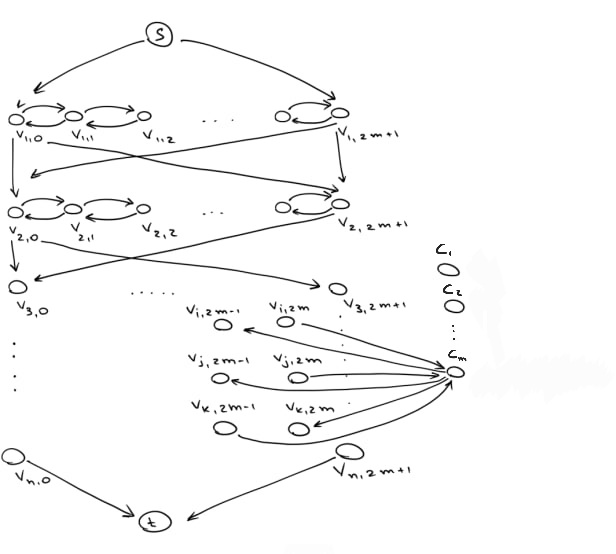
\includegraphics{images/sol11.png} \\
        \text{мал. 2 побудова}
        \end{center}

        \quad Тому ми можемо стверджувати, що граф \(G'\) містить гамільтонів цикл, якщо граф \(G\) містить гамільтонів шлях. Отже, довільний екземпляр задачі \hamcycle зводить до екземпляру задачі \dhampath. З чого можна зробити висновок, що \hamcycle є \(NP\)-складною.\\
        
        \quad Підсумовуючи все вище сказане, маємо, що \hamcycle належить класу \(NP\) і є \(NP\)-складною, тому можна зробити висновок, що \hamcycle є \(NP\)-повною.

        
    \hspace{15cm} \rule{0.7em}{0.7em}
    
    \\
    \quad Тепер, довівши \textit{Твердження 1}, можемо виконати фінальні викладки. Маємо, що \hamcycle належить класу \(NP\) та \nonhamcycle є доповненням задачі \hamcycle, отже задача \nonhamcycle належить класу \(coNP\). Також, врахувавши, що \hamcycle є \(NP\)-повною, можна зробити висновок, що \nonhamcycle є  \(coNP\)-повною.
        

    \section{\normalfontРозв'язок}
    \textcolor{red}{However, for some specific graph classes, there are well-known algorithms for finding solutions. For example, the minimal vertex cover problem for cubic graphs can be solved using the Blossom algorithm. For planar graphs, the Hamilton cycle problem can be solved in polynomial time using the Hopcroft–Tarjan algorithm. Additionally, applications of Approximation algorithms, such as the Christofides algorithm, offer good solutions for specific classes of graphs.}
        \subsection{\normalfontНаявні методи розв'язку}
        \subsection{\normalfontНаявні ефективні часткові розв'язки задачі та модифікацій}

    \section{\normalfontСписок використаної літератури}
    \textcolor{blue}{чи доречно лишати лінки?}
    \begin{thebibliography}{9}
        \item Adrian She, \emph{Hamiltonian Path is NP-Complete}, 2020.
        \item Dan Archdeacon, \emph{An Historical Account of the Non-Hamiltonian Cycle Problem}.
    \end{thebibliography}


    
	\end{spacing}
\end{document}
